\documentclass[main.tex]{subfiles}
\begin{document}
\chapter{Introduction}
\label{ch:intro}
\section{Our Team}
Waterloop is a team of ambitious students from the University of Waterloo who have been working to design and build prototype Hyperloop pods since September 2015 with the goal to compete in SpaceX's Hyperloop Pod Competitions. We hope to represent Canada's leading innovation on the world stage at Competition III.

The team is based in Waterloo, Ontario, Canada’s largest technology innovation hub. Waterloop has members studying in fields ranging from engineering to arts to environment to business, and our members also represent over 20 countries of origin. Our diverse team is united under the common goal of building a pod that cannot only do well in competition, but can eventually be implemented in Canada's transportation infrastructure. We believe Hyperloop has the potential to link together the economy and shrink the world in a faster, cleaner, and more efficient way.

We are excited to build cutting-edge technology with the potential to revolutionize - or even trivialize - the concept of distance. On a personal level, it has been an extraordinary experience teaching and learning technical and administrative skills, creating strong organizational and engineering practices, and most of all, engaging in amazing teamwork. We are also proud to be actively promoting programs that will bring our own life-changing experiences to a wider community, including work with HeForShe Waterloo and hosting educational events to promote the importance of STEM for Canada's future. We hope to be a leader in Canada's surge back into the forefront of innovation.

\subsection{Administrative Facts}
\begin{itemize}
\item Performed a complete rebranding, resulting in the logo which can be seen at the bottom of each page.
\item Confirmed over \$30,000 in sponsorship, with much more under discussion.
\item Reached nearly 4000 likes on Facebook, and less than a week after opening recruitment have received almost 50 applications.
\item Gained support at many levels of the University administration through periodic pod showcases and tours.
\end{itemize}

\subsection{Team Members Fall 2017}
Due to the UWaterloo co-op system, our team rotates approximately every four months.

\begin{multicols}{3}
	\centering{\large{Directors}}
    \begin{itemize}[label={},noitemsep]
        \item Clive Chan, Technical
        \item Jason Pan, Administrative
    \end{itemize}
    \centering{\large{Advisors}}
    \begin{itemize}[label={},noitemsep]
        \item Serhiy Yarusevych, Faculty Advisor
        \item Victor Qian, Alumnus/Advisor
    \end{itemize}
    \centering{\large{Integration Leads}}
    \begin{itemize}[label={},noitemsep]
        \item Ben, Faculty Advisor
        \item Jimbo, Alumnus/Advisor
    \end{itemize}
\end{multicols}
\centering{\LARGE{Technical Teams}}
\begin{multicols}{3}
    \centering{\large{Mechanical}}
    \begin{itemize}[label={},noitemsep]
    \item \textbf{Jimmy Zhou, Mechanical Lead}
    \item \textbf{Ben Tonita, Mechanical Lead}
    \item \textbf{Donovan Kwong, Friction Drive}
    \end{itemize}
    \centering{\large{Software}}
    \begin{itemize}[label={},noitemsep]
    \item \textbf{Deep Dhillon, Lead}
    \item \textbf{Ruslan Nikolaev, Lead}
    \end{itemize}
    \centering{\large{Electrical}}
    \begin{itemize}[label={},noitemsep]
    \item \textbf{Chawthri Kanagarasa, Lead}
    \end{itemize}
\end{multicols}
\centering{\LARGE{Administrative Teams}}
\begin{multicols}{3}
    \centering{\large{Sponsorship}}
    \begin{itemize}[label={},noitemsep]
    \item \textbf{Nicholas Jelich, Lead}
    \end{itemize}
    \centering{\large{Media}}
    \begin{itemize}[label={},noitemsep]
    \item \textbf{Natalia Zigante, Lead}
    \end{itemize}
    \centering{\large{Finance}}
    \begin{itemize}[label={},noitemsep]
    \item \textbf{Nafee Hasan, Lead}
    \end{itemize}
\end{multicols}
\begin{itemize}
    \item Administrative Leads: Nicholas Jelich, Natalia Zigante, Nafee Hasan, Aditya Arora, Emile Patry
    \item Technical Leads: William Ngana, Deep Dhillon, Ruslan Nikolaevra, Urooj Khaleeli, Jimmy Zhou, Benjamin Tonita, Chawthri Kanagarasa, Lily Hwang
\end{itemize}

\centering{\LARGE{Team Roster}}
\begin{multicols}{4}
 \begin{itemize}[label={},noitemsep]
     \item {Aayush Sharma}
     \item {Abdelrahman Ayad}
     \item {Aditya Arora}
     \item {Adrian Fagarasanu}
     \item {Ahmed Al-Hasani}
	 \item {Ambareesh Balaji}
     \item {Amy Sun}
	 \item {Anthony Fabian}
     \item {Archer Zhang}
	 \item {Armanit Garg}
     \item {Arnav Garcha}
	 \item {Attilio Ravani}
     \item {Ayush Kapur}
	 \item {Ben Tonita}
     \item {Benjamin Li}
	 \item {Bob Wei}
     \item {Callum McCracken}
	 \item {Casey Garcia}
     \item {Chawthri Kanagarasa}
	 \item {Chun Hang Lau}
     \item {Clive Chan}
	 \item {Colin Batchellor}
     \item {Connor Nicholls}
	 \item {Cyril Vaidhyan}
     \item {Dallyn Wynnychuk}
	 \item {Daniel Ingriselli}
     \item {Daniyal Shaikh}
	 \item {Deep Dhillon}
     \item {Donovan Kwong}
	 \item {Edmond Lu}
     \item {Edwin Zhang}
	 \item {Egemen Guray}
     \item {Emile Patry}
	 \item {Emrys Halbertsma}
     \item {Eniife Elebute}
	 \item {Gianni Recupero}
     \item {Greg Hill}
	 \item {Griffin Barniutt}
     \item {Griffin Keglevich}
	 \item {Heather D'Souza}
     \item {Ibrahim Irfan}
	 \item {Imad Azzam}
     \item {Isabel Zhu}
	 \item {James Lu}
     \item {James Ro}
	 \item {Jason Pan}
     \item {Jeff Niu}
	 \item {Jenarth Jegatheeswaran}
     \item {Jimmy Zhou}
	 \item {Jonathan Lee}
     \item {Jordan Lin}
	 \item {Justin Gorvett}
     \item {Justin Hammond}
	 \item {Justin Pu}
     \item {Justin Schaper}
	 \item {Kaeun Kim}
     \item {Kelvin Tezinde}
	 \item {Kunal Jhaveri} 
	 \item {Laura Chambers}
     \item {Lily Hwang}
	 \item {Loic Murumba}
     \item {Mathieu Godin}
	 \item {Melissa Tran}
     \item {Monica Chung}
	 \item {Nafee Hasan}
     \item {Namitra Kalicharran}
	 \item {Natalia Zigante}
     \item {Natasha Poley}
	 \item {Navraj Singh Chhina}
     \item {Navreet Dhillon}
	 \item {Neil McClean}
     \item {Nicholas Jelich}
	 \item {Nicole Rosario}
     \item {Noah Ford}
	 \item {Pascal Voyer-Nguyen}
     \item {Promit Barua}
	 \item {Ruslan Nikolaev}
     \item {Saif Hafeez}
	 \item {Sam MacLeod}
     \item {Shubham Patil}
	 \item {Shun Rao}
     \item {Stefan Sing}
	 \item {Stephanie Mills}
     \item {Turja Aninda}
	 \item {Tushar Sekhri}
     \item {Tyler Zhang}
	 \item {Urooj Khaleeli}
     \item {Victor Qian}
	 \item {William James Ngana}
     \item {William Xian}
	 \item {William Yan}
     \item {Yazan Obeidi}
	 \item {Yi Dong}
     \item {Yingning Gui}
	 \item {Zhaoxin Zhang}
     \item {Ziyang Huang}
	 \item {Steven Kozachuk}
\end{itemize}
\end{multicols}

\begin{flushleft}
\subsection{Sponsors}
Thanks to all our sponsors, past and present

\begin{multicols}{3}
    \begin{itemize}[label={},noitemsep]
    \item \textbf{Babylon VR}
    \item \textbf{BALLUFF}
    \item \textbf{Boko}
    \end{itemize}
\end{multicols}

\begin{multicols}{3}
\begin{itemize}[label={},noitemsep]
    \item \textbf{Camino modular systems}
    \item \textbf{Caro Systems}
    \item \textbf{Communitech}
    \end{itemize}
\end{multicols}

\begin{multicols}{3}
\begin{itemize}[label={},noitemsep]
    \item \textbf{Dassault Systems}
    \item \textbf{Eagle CAD}
    \item \textbf{GroveWare}
    \end{itemize}
\end{multicols}

\begin{multicols}{3}
\begin{itemize}[label={},noitemsep]
    \item \textbf{Heins Management, Consulting Inc.}
    \item \textbf{IBI}
    \item \textbf{iDream Labs}
    \end{itemize}
\end{multicols}

\begin{multicols}{3}
\begin{itemize}[label={},noitemsep]
    \item \textbf{Infinity Testing}
    \item \textbf{Inksmith}
    \item \textbf{Javelin}
    \end{itemize}
\end{multicols}

\begin{multicols}{3}
\begin{itemize}[label={},noitemsep]
    \item \textbf{Kik}
    \item \textbf{League}
    \item \textbf{Leggett and Platt}
    \end{itemize}
\end{multicols}

\begin{multicols}{3}
\begin{itemize}[label={},noitemsep]
    \item \textbf{LOT}
    \item \textbf{Maplesoft}
    \item \textbf{Masrio Architects}
    \end{itemize}
\end{multicols}

\begin{multicols}{3}
\begin{itemize}[label={},noitemsep]
    \item \textbf{Miltera}
    \item \textbf{MMOSER Associates}
    \item \textbf{Naylor}
    \end{itemize}
\end{multicols}

\begin{multicols}{3}
\begin{itemize}[label={},noitemsep]
    \item \textbf{Paypal}
    \item \textbf{Phidon}
    \item \textbf{Routes Transport Group}
    \end{itemize}
\end{multicols}

\begin{multicols}{3}
\begin{itemize}[label={},noitemsep]
    \item \textbf{Sandford Fleming Foundation}
    \item \textbf{Silver Star}
    \item \textbf{Waterloo Architecture Graduates}
    \end{itemize}
\end{multicols}

\begin{multicols}{3}
\begin{itemize}[label={},noitemsep]
    \item \textbf{Sourced}
    \item \textbf{Sustainable TO}
    \item \textbf{University of Waterloo}
    \end{itemize}
\end{multicols}

\begin{multicols}{3}
\begin{itemize}[label={},noitemsep]
    \item \textbf{UW Faculty of Engineering}
    \item \textbf{UW Faculty of Science}
    \item \textbf{UW EngSoc}
    \end{itemize}
\end{multicols}

\begin{multicols}{2}
\begin{itemize}[label={},noitemsep]
    \item \textbf{WEEF}
    \item \textbf{William J. Pristanski}
    \end{itemize}
\end{multicols}

\subsection{Acknowledgements}

\begin{itemize}
    \item Advisors: Serhiy, Victor
    \item Waterloo Formula Electric for guidance on embedded and electrical
    \item Sandra \& Sedra Student Design Centre
    \item Various other things
\end{itemize}
\section{History}
\begin{itemize}

\item Summer 2015:
\begin{itemize}
    \item Assemble the Team.
    \item Officially registered as a University of Waterloo Student Engineering Team.
\end{itemize}

\item Fall 2015:
\begin{itemize}
    \item Preliminary design briefing and evaluation by SpaceX. One of the 1200 teams entering the competition.
\end{itemize}

\item Winter 2016:
\begin{itemize}
    \item Final design briefing and evaluation by SpaceX.
    \item Hyperloop Design Weekend at Texas A\&M. One of the 31 teams around the world to advance.
\end{itemize}

\item May 2016:
\begin{itemize}
    \item Subsystem R\&D and feasibility analysis.
    \item Granted a private workshop at the Sedra Smith Design Centre at the University of Waterloo.
\end{itemize}

\item June 2016:
\begin{itemize}
    \item Designing and building rigs for subsystem testing - air levitation, eddy current braking, operating electronics in a vacuum.
\end{itemize}

\item August 2016:
\begin{itemize}
    \item Parts sourcing.
    \item Frame fabrication.
    \item Construction of a low speed test track.
    \item Finalizing Goose I subsystem design.
\end{itemize}

\item October 2016:
\begin{itemize}
    \item Achieved air levitation.
    \item Development of embedded and communication systems.
    \item Vacuum chamber testing.
    \item Launching a Kickstarter campaign to supplement sponsorship.
\end{itemize}

\item November 2016:
\begin{itemize}
    \item Successfully raised CA\$43,416 with 507 backers on Goose I Kickstarter campaign.
\end{itemize}

\item December 2016:
\begin{itemize}
    \item High speed performance testing.
    \item System optimization.
    \item Reliability and safety testing.
\end{itemize}

\item January 2017:
\begin{itemize}
    \item Attending SpaceX competition with Goose I pod.
\end{itemize}

\item February 2017:
\begin{itemize}
    \item Analyzing feedback from the SpaceX competition.
\end{itemize}

\item March 2017:
\begin{itemize}
    \item Beginning the build of Goose II pod. Working on overall system improvements and overhaul of multiple subsystems based on feedback from competition.
\end{itemize}

\item May 2017:
\begin{itemize}
    \item Developing a brand new embedded and communication systems.
    \item Completing the assembly of Magnetic Wheels for Goose II.
    \item Starting Goose II shell design process.
    \item Starting the final assembly of the pod.
\end{itemize}

\item June 2017:
\begin{itemize}
    \item Vibrational testing of the Goose II to find and eliminate any resonance frequencies.
    \item Testing new embedded systems elements in vacuum.
    \item Integrating required sensors into embedded systems.
    \item Testing communication systems and data visualization on front-end.
    \item Completing static and dynamic levitation tests.
\end{itemize}

\item July 2017:
\begin{itemize}
    \item Goose II unveil.
    \item Beginning preparations for SpaceX Competition 2.
    \item Implementing redundancy checks and safety enhancing features in software.
    \item Second vibrational testing to tune shock absorption for competition.
\end{itemize}

\item August 2017:
\begin{itemize}
    \item Tuning speed controllers for Magnetic Wheels.
    \item Finalizing internal wiring of the pod.
    \item Completing required administrative arrangements for the competition and transportation of the pod to SpaceX headquarters in California.
    %\item Major Mcdonald's run.
    \item Shipping the pod to California.
    \item Attending SpaceX Competition 2.
\end{itemize}

\end{itemize}

\chapter{Top-Level Design}
\label{ch:top-level-design}
Labeled CAD (Exploded? Semitransparent? Color coded?)\\

Our pod design process for Competition III began with the goal of building the fastest possible pod. Based purely on specific power and energy of lithium ion batteries (and perhaps supercapacitors), it is theoretically possible to achieve speeds above Mach 1 within the 1-mile Hyperloop test track. Our pod this year is designed to achieve 100 m/s, and we are gradually working towards higher and higher speeds for future competitions.


\section{Summary of design}
Our pod consists of the following major components:
\begin{itemize}
    \item Propulsion: Friction drive (wheels)
    \item Braking: High speed eddy current braking, low speed caliper brakes
    \item Lateral stability: Freely spinning wheels
    \item Frame: Aluminum ladder frame
\end{itemize}
Uniqueness/Novelty\\
The Pod for the third competition differentiates itself from the previous one, primarily due to the incorporation of the propulsion system. This change has
Changes from PDB and reasoning for changes\\
If reusing a system in whole or part, explain changes\\

\subsection{Size and Mass}
The size of the pod is primarily dictated by the size of the propulsion system and the size of the I-beam.\\
  The mass of the pod depends on the individual mass of each subsystem, as seen in \reftab{table:mass}. The overall mass of the pod should be approximately 150 kilograms.

\begin{table}
\centering
\begin{tabular}{@{}lr@{}}
	\toprule Subsystem & Mass of Subsystem (\si{kg}) \\ \midrule
    Friction Drive & 55.8 \\
    Frame & 19.0 \\
    Electrical & 23.5 \\
    Embedded Systems & unknown \\
    Shell & 12.0 \\
    Eddy Current Braking & 27.0 \\
    Lateral & 10.1 \\
\end{tabular}
  \caption{Mass of individual subsystems}
  \label{table:mass}
\end{table}

Overall weight distribution/Centre of mass\\
The cross-section of the pod is small enough that aerodynamic effects like the Kantrowitz limit\\
are negligible (IS THIS SENTENCE OUT OF PLACE? TODO).\\

\subsection{Energy Storage and Usage}
Where is energy stored onboard the pod?
\begin{itemize}
    \item Huge batteries
    \item Air tanks
    \item Lateral/EC Brakes springs?
\end{itemize}
Where is energy used onboard the pod?
\begin{itemize}
    \item Friction drive
    \item Electronic systems (electrically isolated)
\end{itemize}

\subsection{Overall pod thermal profile}
How are various parts of the pod cooled? (summarize) TODO

\subsection{Predicted Pod trajectory}
\reffig{fig:pod-trajectory-profile} describes the trajectory of the pod while braking.\\
\begin{figure}
	\centering
	\begin{subfigure}{0.4\textwidth}
        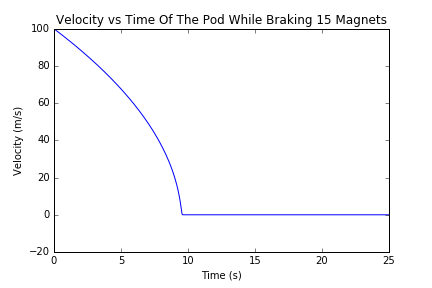
\includegraphics[width=\linewidth]{images/velocity_time_graph}
        \caption{Velocity Profile During Braking}
        \label{fig:velocity-profile}
    \end{subfigure}
    \begin{subfigure}{0.4\textwidth}
        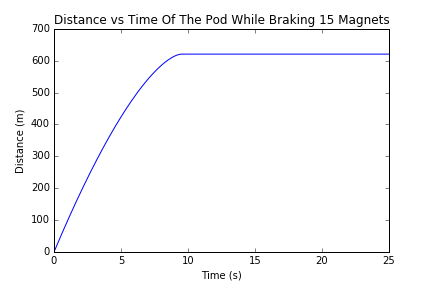
\includegraphics[width=\linewidth]{images/distance_time_graph}
        \caption{Distance Travelled During Braking}
        \label{fig:distance-profile}
    \end{subfigure}
    \caption{Pod Trajectory Profile During Braking}
    \label{fig:pod-trajectory-profile}
\end{figure}
\subsection{Loading and Unloading Plan}
Due to the pod being relatively lightweight – approximately 150 kilograms, the pod can simply be moved and lifted by 10 people. Therefore, moving to and away from the Hyperloop competition is not a large safety concern.

\section{Scalability}
Our pod design seeks to be the simplest possible design for a Hyperloop. However, it is difficult to scale to high-subsonic speeds for several reasons.
In order to fully do so, the team will eventually need to gain experience with high power systems, high speed stability, and braking systems on a larger scale.\\

Preliminary analysis on scalability to an operational Hyperloop needs to be done with respect to:
\begin{itemize}
    \item System size (increased tube length, tube diameter, and Pod size)
    \item Cost (both production and maintenance)
    \item Estimated Pod mass and cost if built full-scale
    \item Maintenance (e.g. not requiring specialized alignment tools, hot-swappable subsystems)
    \item Power, cooling, safety, etc.
    \item Propulsion effectiveness
\end{itemize}
\end{flushleft}
\end{document}